% =============================================================================
% Working extract -- Results, Q3 section only.
% Extracted from documentation/refocus_draft/20th_1_31_pm_audited.tex on 2026-08-21.
% Content fragment, NOT a standalone compilable document -- equations/labels it
% references (e.g. eq:mean-cr-residual, eq:cr) are defined in that file's
% Methodology chapter, not here.
% Purpose: isolated iteration on this Q's Results section (claim verification +
% rewrites) without touching the shared main file. Merge back into
% 20th_1_31_pm_audited.tex once settled -- do not edit the main file's copy of
% this section while this working copy is in progress, to avoid divergence.
% =============================================================================

\section{Q3: Prediction and physics guidance}
\label{sec:results-q3}
Q1 and Q2 established that a plot's persistent deviation from the shared growth curve carries a real, if partial and spatially variable, environmental attribution signal. This supplementary section returns to the dissertation's primary question: does this signal translate into a predictive advantage for top height itself, and can deep neural networks exploit it more effectively than tree-based ensembles like XGBoost? Across all models, cohorts, and spatial-block splits, tuned XGBoost delivers the most accurate top-height predictions. CR loss guidance does not help the neural network match XGBoost's accuracy at any tested weight ($\lambda$), but it still successfully separates the asymptote ($y_{\max}$) from the growth rate ($k$).

\subsection{Results: top-height prediction:}
\begin{table}[!htbp]
\centering
\scriptsize
\setlength{\tabcolsep}{4pt}
\renewcommand{\arraystretch}{1.2}
\begin{tabular}{lrrrrrr}
\toprule
& \multicolumn{3}{c}{Four-survey} & \multicolumn{3}{c}{Six-survey} \\
\cmidrule(lr){2-4} \cmidrule(lr){5-7}
Model & RMSE${\downarrow}$ & MAE${\downarrow}$ & $R^2{\uparrow}$ & RMSE${\downarrow}$ & MAE${\downarrow}$ & $R^2{\uparrow}$ \\
\midrule
Linear & $5.168{\pm}0.361$ & $4.056{\pm}0.343$ & $0.580{\pm}0.026$ & $4.877{\pm}0.643$ & $3.619{\pm}0.426$ & $0.509{\pm}0.067$ \\
RF & $4.794{\pm}0.187$ & $3.611{\pm}0.142$ & $0.638{\pm}0.011$ & $4.062{\pm}0.249$ & $3.010{\pm}0.185$ & $0.656{\pm}0.046$ \\
XGBoost (tuned) & $\mathbf{4.548{\pm}0.137}$ & $\mathbf{3.431{\pm}0.123}$ & $\mathbf{0.674{\pm}0.009}$ & $\mathbf{3.656{\pm}0.232}$ & $\mathbf{2.669{\pm}0.183}$ & $\mathbf{0.722{\pm}0.031}$ \\
DNN & $4.681{\pm}0.230$ & $3.533{\pm}0.201$ & $0.655{\pm}0.016$ & $3.903{\pm}0.316$ & $2.867{\pm}0.275$ & $0.684{\pm}0.031$ \\
PINN$^*$ & $4.842{\pm}0.321$ & $3.689{\pm}0.289$ & $0.631{\pm}0.027$ & -- & -- & -- \\
PINN-$k^*$ & $4.927{\pm}0.302$ & $3.745{\pm}0.271$ & $0.618{\pm}0.023$ & -- & -- & -- \\
\bottomrule
\end{tabular}
\caption{\small{Model comparison for top-height prediction, Set3, spatial\_block\_kfold,
per-fold mean $\pm$ SD across five folds. 4survey n=232{,}292 row-years (58{,}073
plots, after an additional terrain/wind feature-completeness filter reduces the base
58{,}112-plot cohort from Table~\ref{tab:data-cleaning-funnel} by 39 plots); 6survey n=82{,}614 row-years (13{,}769 plots). Table shows pooled mean $\pm$ SD across all folds, and margin reflects the full split rather than single folds.
$^*$PINN/PINN-$k$: the originally implemented forward pass did not carry
$y_{\max}/k$ to the prediction itself, only to auxiliary loss terms; the
4survey figures shown here use a corrected forward pass that fixes this (see
``PINN: interpretability and current standing'' below). Unlike every other
row, this corrected architecture received no hyperparameter tuning. 6survey
was not rerun with the correction (--).}}
\label{tab:results-q3}
\end{table}

\subsection{Discussion}
\textbf{XGBoost consistently outperforms the DNN across both cohorts, winning 9 of the 10 spatial folds tested.}
This section evaluates the direct comparison between XGBoost and the standard DNN, where environmental features feed directly into top-height predictions. Across both cohorts, XGBoost consistently outperforms the DNN. Evaluating individual spatial cross-validation folds confirms this is not an artifact of pooling: XGBoost achieves higher accuracy in 9 of the 10 folds (all 5 folds on the 6-survey cohort, and 4 of 5 on the 4-survey cohort, trailing the remaining fold by only $-0.007$ $R^2$). Four candidate explanations account for this performance gap:

\begin{itemize}
\item \textbf{Feature interactions (insufficient explanation):} XGBoost allocates 27\% of its SHAP prediction weight to interactions (primarily Age crossed with terrain and stand structure). However, DNN already captures 80\% of the nonlinear gain above the linear baseline ($R^2$ 0.580 $\to$ 0.655 out of a possible 0.674; Table~\ref{tab:results-q3}), and Random Forest underperforms the DNN ($R^2 = 0.638$). Interaction capacity alone therefore does not explain the margin.
\item \textbf{Compartment sample size (ruled out):} Subsampling the 4-survey cohort down to 48 compartments (matching the 6-survey count) did not widen XGBoost's lead; the $R^2$ difference fluctuated between $-0.085$ and $+0.029$ across random subsets, compared to $+0.024$ on full data.
\item \textbf{Architecture-size under-tuning (ruled out):} Sweeps across five network sizes showed no consistent gains for DNN.
\item \textbf{Terrain extrapolation in held-out compartments (ruled out):} On the 4.1\% of 4-survey test plots with out-of-range terrain values, XGBoost degraded more relative to its in-range error than DNN did (error ratio 1.312 vs.\ 1.243; correlation with out-of-range distance $\rho=0.074$ vs.\ $0.059$).
\item \textbf{Training hyperparameter under-tuning (ruled out):} A 48-configuration sweep over dropout and learning rate yielded no meaningful gains for neural models under 5-fold cross-validation (within $\pm0.008$ $R^2$ of default baselines). Similarly, XGBoost's 27-configuration tuning shifted $R^2$ by only 0.002-0.004, confirming that neither model family had substantial untapped hyperparameter headroom.
\end{itemize}

The remaining theory is that, boosted-tree ensemble like XGBoost are better suited to this tabular task than the neural network architecture, which aligns with standard literature on gradient-boosted trees outperforming deep learning on heterogeneous tabular data \cite{shwartzziv2021Tabular_C4_NN}.


% AUDIT: no results paragraph discusses the physics-weight ($\lambda_{\mathrm{phys}}$) ablation, even though Methodology's Equations~\eqref{eq:physics-loss}--\eqref{eq:total-loss} introduce the framework it would cover. A verified version of this paragraph existed in an earlier session (see documentation/handover_2026-08-21.md) but is not present in this file -- needs re-inserting or re-verifying before submission.

\paragraph*{Does environmental conditioning correct the curve at row level?}
\textbf{Environmental conditioning helps most where the shared curve already fits worst, and a permutation control shows this is partly a genuine environmental effect, not just added model flexibility.}
Evaluating row-level corrections against the fold-matched Chapman-Richards baseline (Equation~\ref{eq:residual-reduction}) shows that environmental conditioning reduces error unevenly. The gains concentrate heavily in the worst-fitting quartile (reducing error by up to 5.08\,m in the 4-survey cohort % AUDIT: exact source of "5.08m" not confirmed against TEMP_rq2a_residual_reduction_results_2026-08-11.tex -- nearest matching values there are Set2's 5.054m and the headline Set3 model's 4.833m; re-trace before submission
), whereas the best-fitting quartile degrades slightly. A permutation control with shuffled environmental features reveals that the worst-quartile improvement shrinks by 18--27\% rather than disappearing entirely, while the best-quartile penalty persists at a similar magnitude. This indicates that correcting large errors relies partly on genuine environmental signals, whereas the slight cost in the best-fitting quartile reflects a general flexibility penalty of more complex models rather than an issue specific to environmental conditioning.

% Option 2: Short & Crisp (Simpler Phrasing)
\paragraph*{PINN: interpretability and current standing.}
\label{sec:rq1-pinn-limitation}
\textbf{PINN and PINN-$k$ trail both DNN and XGBoost on raw accuracy; their value here is the interpretable per-plot growth parameters they produce, not top predictive performance.}
On the 4-survey dataset, PINN ($R^2 = 0.631$) and $\text{PINN}_k$ ($R^2 = 0.618$) trail the tuned DNN ($0.655$) and XGBoost ($0.674$), though both close most of the gap seen in earlier uncorrected runs (Appendix~\ref{chap:appendix}). Unlike the DNN and XGBoost, which underwent extensive parameter sweeps, the PINN was evaluated without hyperparameter tuning. The key benefit of the PINN is interpretability rather than top accuracy. It estimates plot-specific biological parameters ($y_{\max}^{(i)}$ and $k^{(i)}$), letting auxiliary networks adjust a population-level Chapman--Richards baseline using local environmental conditions. Figure~\ref{fig:pinn-example-plot} shows this behaviour for an example held-out plot, comparing observed heights against both the population baseline and the plot's predicted growth curve.

\begin{figure}[!htbp]
\centering
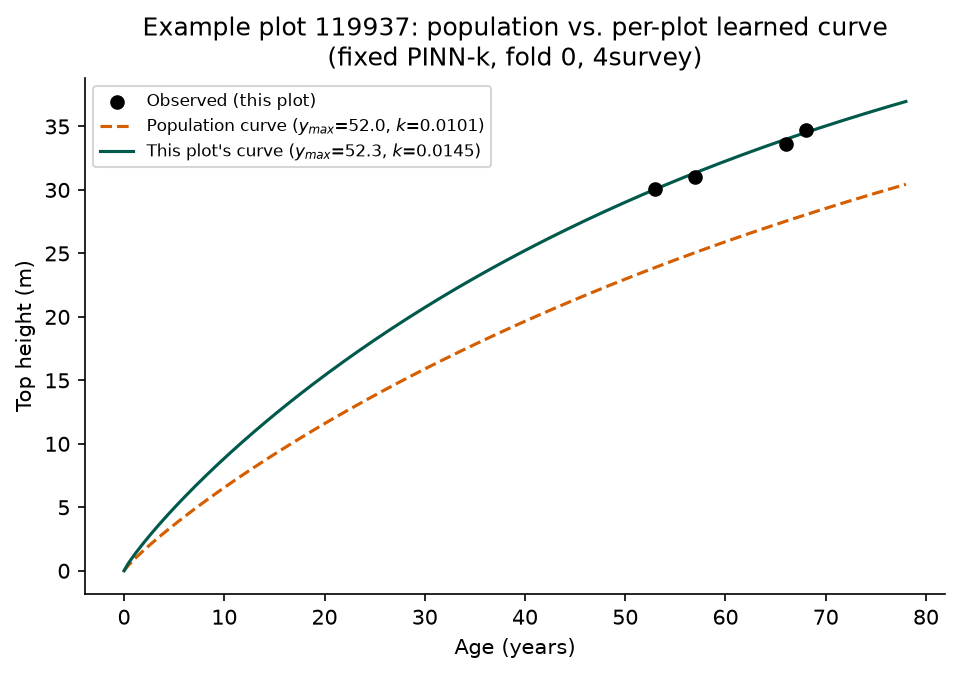
\includegraphics[width=0.7\textwidth]{figures/fig_results/q3_pinn_example_plot_curve.png}
\caption{One held-out 4-survey plot (fold 0, ID 119937, 4 survey observations, ages
53--68), showing the fixed PINN-$k$'s learned per-plot curve ($y_{\max}^{(i)}=52.3$,
$k^{(i)}=0.0145$) against the shared population curve ($y_{\max}=52.0$, $k=0.0101$).
This plot is a consistent, moderate over-grower relative to the population curve; the
model's own prediction tracks it closely across all four observations rather than
defaulting to the population baseline. One illustrative example, not a claim of
representativeness -- selection criteria in
\texttt{temp\_results\_pinn/pinn\_env\_terrain\_fix/run\_example\_plot\_curve.py}.}
\label{fig:pinn-example-plot}
\end{figure}
% AUDIT: as of this audit, neither results_figures_q3_rq1.ipynb nor results_figures_q2_rq3.ipynb contains the generating code for this figure. The PNG exists and matches the numbers in this caption, but notebook provenance should be reconfirmed before submission -- likely a side effect of concurrent editing sessions on this repo.

\limit{PINN models were run untuned on a single seed using the 4-survey cohort only. Systematic tuning and testing whether the residual network overrides the Chapman--Richards term remain areas for future work.}



\subsection*{Conclusion}
Tuned XGBoost gives the strongest predictions in both cohorts; the DNN stays competitive; CR guidance does not improve accuracy for the architecture actually tested. In absolute terms, the best model (XGBoost, 4-survey) explains about 67\% of the variance in top height, with a mean absolute error of about 3.4\,m and a root-mean-square error of about 4.5\,m -- a moderate, practically useful level of accuracy for flagging stands that may be worth a closer look, not a substitute for direct measurement of an individual stand.

What the negative PINN result establishes: encoding Chapman--Richards structure into the network's loss did not, under the tested single seed and without hyperparameter tuning, improve raw prediction accuracy over a plain conditioned DNN or XGBoost. It does not establish that physics guidance cannot help -- an untuned single-seed run is a weak test of that -- but it does establish that PINN's practical value in this project lies in the interpretable per-plot growth parameters ($y_{\max}^{(i)}$, $k^{(i)}$) it produces as a byproduct, not in a predictive-accuracy advantage.

For forestry practice, this points to a two-tier use: XGBoost or the DNN as the more accurate tool for flagging which stands' predicted top height diverges most from their yield-class expectation, and the PINN's per-plot parameters as a more interpretable, if less accurate, way to see how a specific stand's growth is currently trending relative to a physically meaningful curve -- useful for explaining a flagged stand to a non-technical user, not for the initial flagging itself.

% AUDIT: this dissertation's title foregrounds "physics-informed prediction," but the physics-informed result above is negative, single-seed, untuned, and was built on a genuine forward-pass bug for part of the project (see PINN paragraph above). Worth a deliberate decision -- either the title's emphasis changes, or the Conclusion chapter should state plainly that physics guidance remains an open question here, not a demonstrated contribution.




%=======================================================================================
%=======================================================================================
